\documentclass[a4paper,10pt,abstracton]{scrartcl}
\usepackage[utf8]{inputenc}
\usepackage{cite}
\usepackage{hyperref}
\usepackage[italian]{babel}
\usepackage{float}
\usepackage{graphicx}
\usepackage{cleveref}
\usepackage{tikz}

\usetikzlibrary{arrows,shapes,positioning}

\begin{document}

\title{Robby the robot: un approccio collaborativo basato su reti neurali}
\subtitle{Progetto di Fisica dei Sistemi Complessi}

\author{Davide Berardi, Michele Corazza}

\maketitle

\begin{abstract}
	In questa relazione tratteremo il problema di Robby collaborativo,
	un robot che esplora mappe bidimesionali con il fine di ripulirle da
	lattine posizionate sulla alcune celle, esteso dalla presenza di diversi
	robot sulla stessa mappa.
	L'approccio da cui muove questo progetto è basato su tecniche di
	apprendimento puramente genetico.
	Si è invece introdotto un nuovo approccio basato su reti neurali evolute
	geneticamente. Mostreremo come tale approccio conduca a vantaggi
	significativi e sia una soluzione percorribile al problema.
\end{abstract}

\section{Introduzione}
Il problema dell'esplorazione di mappe inizialmente sconosciute, finalizzato 
alla
localizzazione di determinati oggetti, è ben noto in letteratura. Tale scenario
rientra nella branca dell'intelligenza
artificiale e, come molti altri della stessa categoria, può essere
risolto tramite meccanismi puramente descrittivi, i quali 
codificano in un
algoritmo l'esatto comportamento da adottare, oppure meccanismi di apprendimento
i quali selezionano una tattica vincente tramite le performance richieste. In
quest'ultima categoria rientrano, in particolare, gli approcci evolutivi genetici
e basati su reti neurali. I primi, ispirati alla teoria della selezione naturale
di Charles Darwin, evolvono il comportamento atteso selezionando i candidati in
base alla loro capacità di risolvere il problema in esame. Un aspetto cruciale
riguardante tale approccio è la rappresentazione del genoma, che codifica le
caratteristiche di un singolo individuo, utilizzato per evolvere la specie
tramite riproduzione sessuata e mutazione in modo analogo a quanto avviene in
natura.\\

Gli approcci basati su reti neurali sono anch'essi ispirati alla biologia:
essi emulano difatti il comportamento del sistema nervoso centrale animale, nel
quale un segnale elettrico si propaga in una rete di neuroni
consentendo computazioni complesse. Al fine di tarare la rete, è possibile
utilizzare approcci supervisionati, che modificano la rete a posteriori a
partire dagli output desiderati, ed approcci non supervisionati, i quali
evolvono la rete in base alle performance della stessa nella risoluzione del
problema.\\

Sono comunque praticabili approcci ibridi, i quali sono in grado di evolvere
reti neurali tramite algoritmi genetici. Un aspetto cruciale negli approcci
basati su reti neurali con apprendimento non supervisionato o
apprendimento genetico puro è la funzione di \emph{fitness}, la quale deve non
solo codificare la bontà di un comportamento, ma anche guidare l'evoluzione
dell'intero sistema.


\section{Scenario}

\begin{itemize}
 \item Modello
 \item Robby genetico
\end{itemize}
Il problema affrontato riguarda l'utilizzo di un robot, chiamato Robby, il cui 
scopo è quello di pulire una stanza dalla forma quadrata raccogliendo delle lattine.
La mappa entro la quale il Robby si muove consiste di una griglia 
bidimensionale di celle, che ammette solo posizioni intere.
Le lattine vengono quindi posizionate su celle inizialmente ignote al Robby. Si 
suppone che il Robby sia equipaggiato con sensori in grado di distinguere i muri 
che delimitano l'area esplorabile e di individuare l'eventuale presenza di lattine. La distanza 
massima che il Robby può osservare è un parametro variabile, ma è comunque 
limitata. Altrettanto limitato è il numero di passi discreti che il Robby può 
effettuare; l'azione di raccolta delle lattine viene considerata nel conteggio 
totale dei passi effettuati. La disposizione degli oggetti sulla mappa è 
statica, in altre parole non è possibile che compaiano
%(FIXME)
ulteriori lattine durante l'esecuzione.
\\
Rispetto ai possibili spostamenti, il Robby può muoversi solamente
in quattro direzioni, non vengono perciò considerate direzioni espresse in 
forma di angolo. Ciascun passo consente perciò al Robby di spostarsi fra due celle 
adiacenti.
\\
Una modalità possibile per affrontare il suddetto problema consiste 
nell'utilizzo di un approccio puramente genetico; si procede creando una 
mappatura fra le possibili configurazioni della vista e le mosse che il Robby 
può effettuare. Tale mappatura viene evoluta tramite crossover e mutazioni 
casuali, al fine di massimizzarne l'efficienza del Robby.



\section {Obiettivi}
\begin{itemize}
 \item Collaborazione fra robby
 \item Superare l'algoritmo genetico
\end{itemize}

Un approccio interessante rispetto al suddetto problema riguarda la possibilità
di collaborazione fra più di un Robby sulla stessa mappa. Questa modifica
consente di evidenziare eventuali interazioni complesse fra i Robby. Da questo
punto di vista è fondamentale individuare un paradigma di comunicazione
efficiente, in grado cioè di massimizzare lo scambio di informazioni nel modo
più sintetico possibile.\\

Da questo punto di vista, l'approccio genetico puro risulta problematico:
Aumentando il numero di Robby presenti sulla mappa, il numero di configurazioni
considerate dall'algoritmo genetico aumenta in modo esponenziale, rendendo
computazionalmente dispendiosa la ricerca di corrispondenze efficaci fra
configurazioni in input e possibili azioni. Si è deciso pertanto di tentare
un approccio basato su reti neurali. Tale approccio consente infatti di non
mantenere la corrispondenza diretta tra dati in input e azione da intraprendere,
in quanto tali corrispondenze sono codificate direttamente all'interno della
rete. Fra i vari approcci presenti in letteratura, si è scelto di procedere
mediante una soluzione che evolva la rete in modo puramente genetico.


\section{Progettazione}
Al fine di ottenere un'efficiente comunicazione tra i Robby è importante
individuare quali informazioni sia utile scambiare. In quest'ottica si è scelto
di procedere comunicando tra i Robby le rispettive viste locali. A tale
informazione si è scelto inoltre di aggiungere la posizione assoluta del
Robby\footnote{Nel caso in cui la posizione non sia nota, è possibile conoscerla
muovendo il Robby verso un angolo della mappa.}.\\

Si è introdotta in precedenza la volontà di utilizzare una rete neurale per
governare i Robby. Per rete neurale si intende un grafo orientato ai cui archi 
sono associati dei pesi, ed il cui scopo è quello di apprendere una certa 
funzione. Tale approccio è ispirato alla biologia ed in particolare al sistema 
nervoso centrale degli animali. Da una serie di nodi di input il segnale viene 
propagato lungo la rete e ciascun neurone calcola la somma dei valori sui 
propri archi entranti moltiplicati per il peso di ciascun arco. Esistono vari 
modelli per emulare una rete neurale biologica: è possibile per esempio 
utilizzare percettroni, ovvero neuroni che, calcolato il valore in input dai 
propri archi entranti, propagano l'output sui propri archi uscenti solo se esso 
supera una certa soglia. Nella rete da noi implementata si utilizzano invece 
neuroni artificiali veri e propri, che utilizzano una funzione (nel nostro caso 
un sigmoide) per amplificare o ridurre il valore in input e propagarlo 
attraverso la rete.
\\



\begin{figure}
	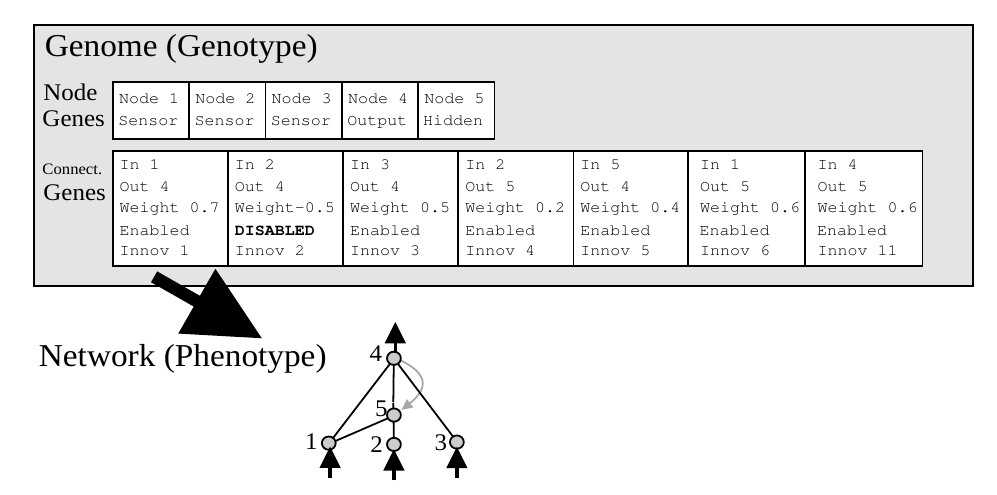
\includegraphics[width=\textwidth]{img/neat-genome.png}
	\caption{Rappresentazione di un genoma in NEAT \cite{stanley2002evolving}}
	\label{fig:neatgenome}
\end{figure}
A tal fine si è individuato l'approccio \emph{NEAT}
(NeuroEvolution of Augmenting Topologies)\cite{stanley2002evolving}. Tale
approccio consente un'evoluzione puramente genetica della rete, compresa la
topologia. Per ottenere tale scopo ciascuna rete viene definita con un
\textbf{genoma} (\cref{fig:neatgenome}) e rappresentata come una sequenza di
nodi e archi (o geni).
A ciascun arco viene inoltre associato un numero monotono crescente denominato
\textbf{innovation}. Tale numero viene utilizzato per stabilire in quale momento
temporale sia stato evoluto il gene ad esso associato. La rappresentazione del
genoma appena descritta consente di misurare una distanza fra i genomi sulla
base della loro similitudine strutturale. Tramite questo meccanismo è possibile
suddividere gli individui in specie entro le quali verrà applicato il crossover.
Il suddetto approccio consente di proteggere i genomi promettenti sulla base
della loro specie permettendo una maggiore varietà genetica ed evitando di
conseguenza l'occorrenza di massimi locali nella ricerca, altrimenti molto
difficili da superare.\\

Al fine di evolvere le reti vengono utilizzati i due approcci tipici degli
algoritmi genetici: \emph{mutazione} e \emph{crossover}.
Le reti vengono mutate con le seguenti modalità:
\begin{description}
	\item[Mutazione dei pesi:] Vengono mutati i pesi dei geni della rete.
	\item[Mutazione delle connessioni:] Viene aggiunto un gene che collega
	due nodi casuali della rete.
	\item[Mutazione dei nodi:] Viene spezzato un collegamento esistente ed
	inserito un nodo collegato ai due capi del suddetto. Il collegamento 
	esistente viene disabilitato.
	(\cref{fig:nodemutate}).
\end{description}

\begin{figure}[H]
	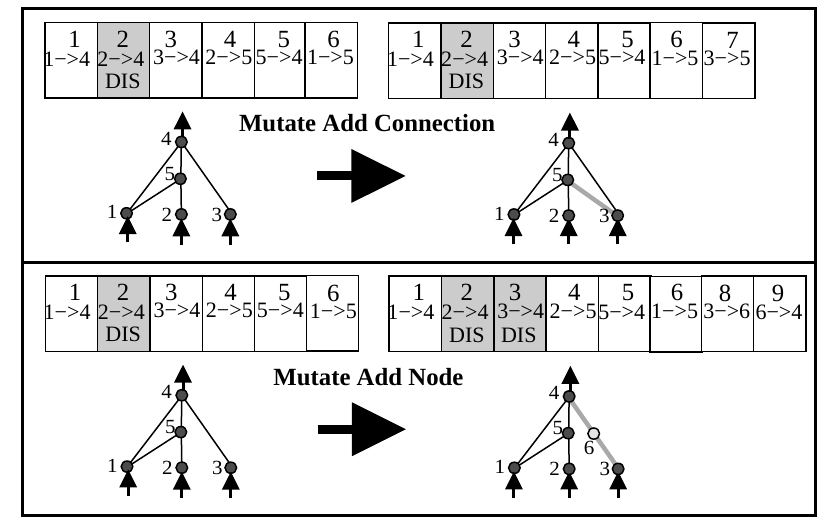
\includegraphics[width=\textwidth]{img/neat-mutation.png}
	\caption{Mutazioni di aggiunta connessioni e nodi
	\cite{stanley2002evolving}.}
	\label{fig:nodemutate}
\end{figure}

Rispetto al meccanismo di crossover, l'approccio NEAT deve far fronte problemi
di compatibilità tra reti con topologie differenti. Viene dunque utilizzata la
distanza fra genomi $\delta$ calcolata nel modo seguente:
\[\delta = \frac{c_1 E}{N} + \frac{c_2 D}{N} + c_3 \overline{W}\]
Dove:
\begin{itemize}
	\item $E$ è il numero dei geni in \textbf{eccesso}, ovvero i geni
	di un genoma che possiedono innovazione maggiore della massima
	innovazione dell'altro genoma considerato.
	\item $D$ è il numero di geni \textbf{disgiunti}, ovvero i geni presenti
	solo in uno dei due individui.
	\item $\overline{W}$ è la differenza media dei pesi dei geni comuni ai
	due individui.
	\item $N$ è il massimo tra il numero dei geni dei due genomi.

	\item $c_1$,$c_2$,$c_3$ sono tre coefficienti utilizzati per tarare
	l'importanza dei tre fattori sopra indicati.
\end{itemize}

Una volta individuate le specie tramite la distanza fra genomi, tra gli
individui della stessa specie viene effettuato il crossover. Viene effettuata
una scansione delle due liste di geni: se il gene risulta in comune viene
ereditato il peso casualmente da uno dei due genitori, mentre i geni in eccesso
o disgiunti vengono aggiunti in ogni caso alla rete risultante 
(\cref{fig:neatcrossover}).

\begin{figure}[H]
	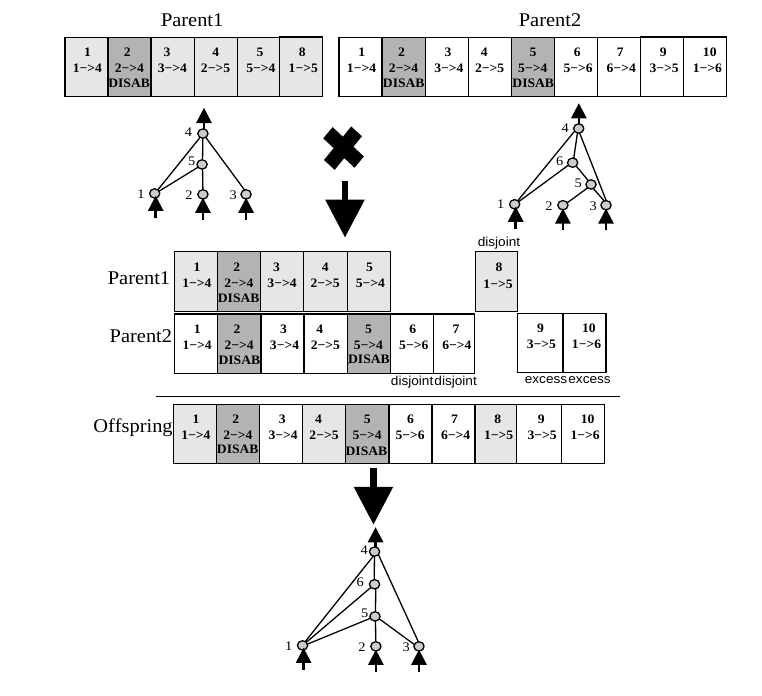
\includegraphics[width=\textwidth]{img/neat-crossover.png}
	\caption{Crossover tra due genomi differenti \cite{stanley2002evolving}.}
	\label{fig:neatcrossover}
\end{figure}



\section{Implementazione}
La struttura di base del programma è stata sviluppata in ottica modulare: a 
run-time è possibile specificare plug-in diversi per gestire la logica dei 
Robby. Tali plug-in devono implementare diverse funzioni: muovere il Robby 
scegliendo la direzione appropriata, generare le strutture dati proprie 
all'algoritmo (es le reti neurali o i genomi per l'algoritmo genetico puro) e 
liberare la memoria allocata in precedenza. La logica di base del programma 
rimane invece invariata, compresa la funzione di fitness. Tale funzione 
deve tenere conto del numero di lattine raccolte e di eventuali fallimenti 
nelle mosse effettuate (es il Robby si muove nella direzione di un muro, oppure 
tenta di raccogliere una lattina su una cella vuota). La fitness è definita 
come segue:
\[\sum\limits_{i=0}^{r} \frac{gc_i}{tc\cdot mn+1}+\frac{sm_i}{t\cdot tc 
\cdot mn + 1}\]
Dove:
\begin{itemize}
 \item $r$ è il numero di Robby presenti su ciascuna mappa;
 \item $gc_i$ è il numero di lattine raccolte dall'i-esimo Robby;
 \item $tc$ è il numero totale di lattine per ciascuna mappa;
 \item $mn$ è il numero totale di mappe;
 \item $sm_i$ è il numero di mosse corrette effettuate dall'i-esimo Robby;
 \item $t$ è il numero di turni totali concessi al singolo Robby.
\end{itemize}
Tale formula considera il successo di tutte le mosse possibili come la raccolta 
di una singola lattina ed incrementa di uno il numero totale di lattine. Il 
valore della funzione è compreso fra 0 e 1, dove 0 è il fallimento totale, 
mentre 1 è il successo totale (tutte le lattine raccolte, nessuna mossa 
sbagliata).
\\
Al fine di consentire la comunicazione dei Robby, viene mantenuta una lista 
globale di messaggi. Ciascun messaggio contiene l'identificatore univoco del 
Robby mittente, la propria vista locale, la propria posizione e l'ultima mossa 
da esso effettuata. Tali informazioni vengono poi combinate dal plug-in 
selezionato per scegliere la strategia migliore.
\\
La vista locale ai Robby è una semplice matrice quadrata che viene popolata dal 
core del programma per mostrare ciò che vede il Robby entro una distanza 
specificata parametricamente. Tale vista non è però quadrata: alcune celle che 
sarebbero incluse in una vista quadrata sono più distanti dal Robby rispetto al 
raggio specificato. Per ovviare a tale problema si è scelto di procedere 
utilizzando il seno discreto per distinguere le celle visibili in questo modo:
\[height(n)=\lfloor r \cdot sin(n\cdot\frac{\pi}{2\cdot r})\rfloor \]
Dove:
\begin{itemize}
  \item $r$ è il raggio del cerchio da generare; 
  \item $n$ è il valore intero che rappresenta la distanza tra il punto in 
  esame sull'asse delle ascisse e il centro, ed è quindi compreso fra 1 e r.
\end{itemize}
Si procede iterando n per calcolare quante celle considerare sull'asse delle 
ordinate sopra alla cella individuata da n. Si ottiene così un quarto di 
cerchio, ed è quindi possibile ruotarlo per ottenere l'intero cerchio discreto.
Una volta ottenuto tale cerchio, le celle al suo interno vengono popolate con 
valori interi che ne rappresentano lo stato(vuoto, lattina, Robby). Le celle 
esterne che sono presenti sulla matrice quadrata vengono impostate come 
sconosciute e non sono considerate dall'algoritmo.
\\
Per implementare la vista globale (detta anche known map) prima di ciascun 
turno vengono controllate le viste locali dei Robby e vengono applicate sulla 
mappa globale le informazioni da esse ricavate. Si ottiene così una vista
globale della mappa nella quale le celle sono sconosciute, vuote o contenti
lattine.
\\

Rispetto all'approccio NEAT classico si sono rese necessarie alcune modifiche
per adattare la tecnica al problema in esame. Rispetto alla creazione iniziale
della rete, nell'articolo originale\cite{stanley2002evolving} le nuove reti
vengono inizializzate come completamente connesse. Nell'implementazione
presentata si è scelto di procedere con reti inizialmente vuote (prive di
archi) al fine di consentire la ricerca di una rete che abbia una struttura
minimale.\\

Rispetto alla evoluzione topologica, l'algoritmo NEAT genera reti che possono
contenere cicli. Tali reti, che vengono dette ricorrenti (\emph{recurrent neural
network}), offrono vantaggi espressivi soprattutto per problemi nei quali ci sia
la necessità di mantenere una ``memoria" all'interno della rete, che pertanto
non viene azzerata tra due esecuzioni. Tale struttura risulta molto adatta a
gestire un flusso continuo di dati. Tuttavia, rispetto al problema in esame,
tale struttura della rete non offre vantaggi e introduce complessità
computazionale nell'attivazione della rete, che deve essere strutturata per
evitare l'occorrenza di cicli infiniti che farebbero altrimenti divergere
l'intero algoritmo. Per ovviare a tale problema si è esteso l'algoritmo NEAT per
impedire la creazione di cicli durante l'evoluzione della rete. A tal fine si è
associata a ciascun nodo una frazione, che indica il livello a cui il nodo
appartiene. Tali valori sono compresi tra 0 e 1 e vengono considerati durante
la \emph{mutazione delle connessioni} e la \emph{mutazione dei nodi}. Durante la
mutazione delle connessioni i livelli dei due nodi adiacenti all'arco da inserire
vengono controllati e, nel caso in cui la connessione sia orientata dal livello
più alto verso il più basso viene invertito il verso dell'arco. Nel caso in cui
i due nodi siano sullo stesso livello l'arco non viene aggiunto. Durante la
mutazione dei nodi il valore del nuovo nodo viene calcolato come la il valore
medio tra i due livelli fra cui verrà inserito (\cref{fig:mutatefraction}).
Tale approccio introduce un ordinamento totale fra livelli, impedendo la
creazione di cicli senza aumentare la complessità computazionale.

\begin{figure}
	\centering
	\begin{tikzpicture}[
		->,
		input node/.style={circle, draw, thick, fill=green!20,minimum size = 7mm},
		hidden node/.style={circle, draw, thick, fill=blue!20,minimum size = 7mm},
		output node/.style={circle, draw, thick, fill=red!20,minimum size = 7mm},
		new node/.style={circle, draw, thick, fill=purple!40,minimum size = 7mm},
		dummy node/.style={circle, thick}
	]
		\node[dummy node] (d1) {};
		\node[dummy node,below of=d1] (d2) {};
		\node[dummy node,below of=d2] (d3) {};
		\node[dummy node,below of=d3] (d4) {};

		\node[input node,right of=d1,xshift=20pt] (i1) {a};
		\node[input node,below of=i1] (i2) {b};
		\node[input node,below of=i2] (i3) {c};
		\node[input node,below of=i3] (i4) {d};

		\node[hidden node,right of=i2,xshift=100pt] (h1) {f};
		\node[hidden node,right of=i3,xshift=100pt] (h2) {g};

		\node[output node,right of=h1,yshift=13pt,xshift=40pt] (o1) {h};
		\node[output node,below of=o1] (o2) {i};
		\node[output node,below of=o2] (o3) {j};

		\node[dummy node,right of=o1, xshift=25pt] (do1) {};
		\node[dummy node,below of=do1] (do2) {};
		\node[dummy node,below of=do2] (do3) {};

		\foreach \i in {1,...,4} {
			\draw[<-] (i\i) -- (d\i) node[above,xshift=0.75cm] {Input \i};
		}

		\draw[->,very thick,red] (i1) -- (h1) {};
		\draw[->] (i2) -- (h1) {};
		\draw[->] (i3) -- (h2) {};
		\draw[->] (i4) -- (h2) {};

		\draw[->] (h1) -- (o3) {};
		\draw[->] (h1) -- (o2) {};
		\draw[->] (h2) -- (o1) {};

		\node[new node,right of=i1,xshift=40pt] (n1) {n};
		\draw[->,very thick,green] (i1) -- (n1) {};
		\draw[->,very thick,green] (n1) -- (h1) {};

		\foreach \o in {1,...,3} {
			\draw[<-] (do\o) -- (o\o) node[above,xshift=1cm] {Output \o};
		}

		\node[dummy node, above of=i1,text width=1cm, align=center]
		(lin) {Level 0};
		\node[dummy node, right of=lin,text width=1cm,align=center,
		xshift=40pt] (lhi) {Level $\frac{1}{4}$};
		\node[dummy node, right of=lin,text width=1cm,align=center,
		xshift=100pt] (lhi) {Level $\frac{1}{2}$};
		\node[dummy node, right of=lhi,text width=1cm,align=center,
		xshift=40pt] (lou) {Level 1};

		
	\end{tikzpicture}
	\caption{Mutazione di un nodo con il meccanismo delle frazioni. Dopo aver
	selezionato l'arco $(a,f)$ viene aggiunto il nodo $n$ e viene posizionato su
	un livello intermedio fra 0 e $\frac{1}{2}$. Il nuovo livello ha quindi
	valore $\frac{1}{4}$. È rappresentato in rosso l'arco disabilitato e in
	verde i nuovi archi.}
	\label{fig:mutatefraction}
\end{figure}




\section{Valutazione e Sviluppi Futuri}
Per valutare il comportamento della rete si sono utilizzate 100 mappe quadrate 
di lato 10 e di lato 5. Il numero di lattine selezionato è stato scelto in 
maniera proporzionale fra le mappe ed è quindi 50 per le mappe di lato 10 e 13 
per le mappe di lato 5. Gli altri parametri sono stati scelti tramite varie 
esecuzioni di prova per valutarne l'impatto sulla performance. Il numero di 
passi che i Robby possono effettuare è stato selezionato per impedire la 
strategia banale che attraversa l'intera mappa per esplorarla e raccogliere le 
lattine. Da test che non verranno qua analizzati in dettaglio è emerso che con 
un numero sufficiente di round il sistema è in grado di raccogliere fino al 
99\% delle lattine.
\\
Nei test da noi effettuati, contrariamente a quanto atteso, l'utilizzo della 
vista globale non conduce significativi miglioramenti nelle performance del 
sistema. La ragione di tale inefficienza è probabilmente da ricondurre alla 
incapacità della rete di apprendere il significato del valore contenuto 
nelle celle della known map, che assumono valori variabili nel tempo. Le celle 
lontane dal Robby sono infatti sconosciute finché non vengono osservate e tale 
comportamento non permette un apprendimento efficace.
\\
Riportiamo in seguito una visualizzazione grafica del comportamento del 
programma durante 4000 generazioni, su mappe di lato 10 e di lato 5 con due
Robby presenti sulla mappa:
\begin{figure}[H]
\centering
\begin{minipage}{.45\textwidth}
	\centering
	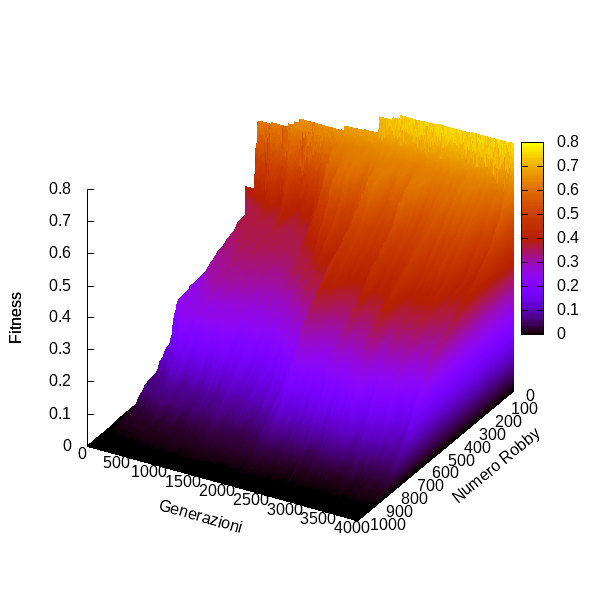
\includegraphics[width=\textwidth]{img/graph10x10.png}
\end{minipage}
\begin{minipage}{.45\textwidth}
	\centering
	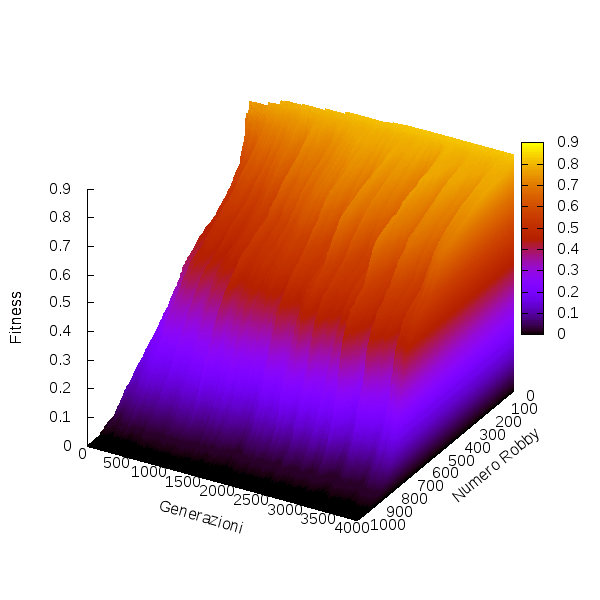
\includegraphics[width=\textwidth]{img/graph5x5.png}
\end{minipage}
\caption{Risultato di 4000 generazioni su mappe di lato 10 (a sinistra) e 5 (a
destra).}
\end{figure}

Come si nota dai grafici, il comportamento dei Robby è quello atteso e la
migliore rete raggiunge valori di fitness di circa $0.8$ corrispondente
all'$80\%$ di lattine raccolte. L'algoritmo è stato inoltre valutato su 100 mappe
non utilizzate nella precedente fase di training. Su mappe di lato 5 ha
raggiunto valori di fitness pari a $0.81$ mentre per mappe di lato 10 valori
pari a $0.78$.  La funzione di fitness sulla mappa più piccola
ha una crescita più rapida che conduce a valori leggermente più alti a causa
del minor spazio di ricerca sulla mappa.\\

Per valutare l'impatto della vista globale presentiamo ora i risultati di 4000
generazioni, su mappe di lato 10 con due Robby:

\begin{figure}[H]
\centering
	\centering
	% XXX: Metti known map!!!
	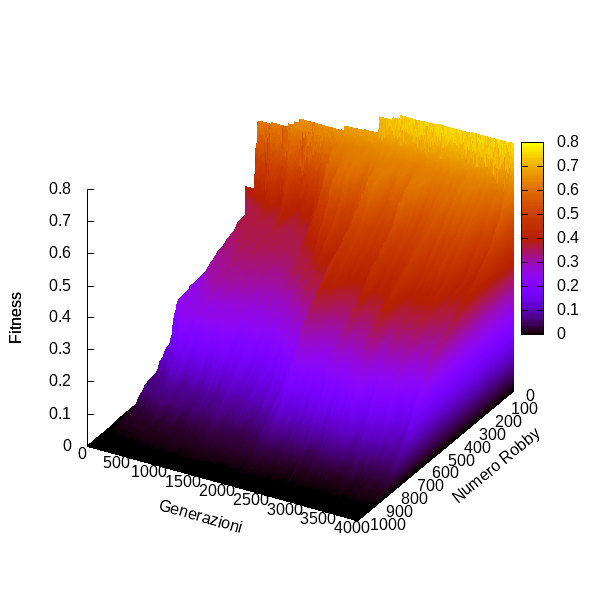
\includegraphics[width=.75\textwidth]{img/graph10x10.png}
\caption{Risultato di 4000 generazioni utilizzando la vista globale su mappe di lato 10.}
\end{figure}

Come facilmente osservabile dal grafico la known map non consente un
apprendimento efficace, specialmente confrontando l'andamento della fitness con
e senza la vista globale.\\

Rispetto ai risultati ottenuti con la vista globale, è lecito chiedersi se sia
possibile implementare un approccio ibrido tra la vista locale con scambio di
messaggi e la vista puramente globale. Questo approccio potrebbe migliorare la
crescita delle reti, consentendo l'algoritmo di superare massimi locali e
\emph{plateau} in modo più efficace. In tal senso un approccio possibile è
l'utilizzo di due insiemi di reti, le une basate su viste locali e le altre su
viste globali. Ciò renderebbe possibile l'utilizzo delle prime per fornire
valori da utilizzare in un apprendimento supervisionato per le seconde. In
alternativa si potrebbe mantenere una memoria di uno storico delle viste locali
precedenti.\\

Un aspetto non trattato in questa relazione è il confronto degli approcci
presentati con l'algoritmo genetico puro. La nozione di posizione, che
risulta di complessa implementazione per l'approccio genetico puro, dovrebbe
condurre a miglioramenti sensibili.



\section{Conclusioni}
In conclusione, abbiamo mostrato come sia possibile utilizzare il meccanismo NEAT
per implementare soluzioni al problema presentato. Abbiamo descritto due
approcci diversi per fornire informazioni alla rete neurale. Tramite le reti
neurali è infatti possibile utilizzare informazioni sulla posizione del Robby
da integrare con le viste locali, oppure una vista globale della mappa. Tali
soluzioni risultano facilmente implementabili su reti neurali, ma introducono
problemi di scalabilità non banali per l'algoritmo genetico puro. Rispetto ai
risultati ottenuti, la valutazione non può che essere positiva per quanto
riguarda le viste locali, in quanto i valori di fitness ottenuti risultano
commisurati al numero di turni concessi ai Robby. A differenza della vista
locale la known map ha condotto a risultati deludenti essendo particolarmente
soggetta a massimi locali e \emph{plateau}. Nonostante i buoni risultati vi è
spazio per ulteriori miglioramenti, in particolare per integrare informazioni
globali che migliorino le performance.



\bibliography{core/biblio}
\bibliographystyle{alpha}

\end{document}
